\section{Determining a simple DE from a description}

\subsection*{Resources}
\begin{itemize}
    \item Text: \url{http://tutorial.math.lamar.edu/Classes/DE/Definitions.aspx}
    \item Book: Chapter 1.2
\end{itemize}

\subsection*{Challenge}
Newton's law of cooling states that the rate of cooling of an object is proportional to the temperature difference with the ambient surroundings. (a) Write a differential equation describing this situation. (b) Assuming a proportionality constant of \num{0.2} \si{/hour}, what is the rate of temperature change when the object is at \SI{30}{\degreeCelsius}?

\subsection*{Solution}
\six{\degreeCelsius/hour}

\hash{q}{078383}




%%%%%%%%%%%%%%%%%%%%%%%%%%%%%%%%%
\newpage
%%%%%%%%%%%%%%%%%%%%%%%%%%%%%%%%%
\section{Direction (Slope) fields}

\subsection*{Resources}
\begin{itemize}
    \item Text: \url{http://tutorial.math.lamar.edu/Classes/DE/DirectionFields.aspx}
    \item Video 1: \url{https://www.khanacademy.org/math/differential-equations/first-order-differential-equations/differential-equations-intro/v/creating-a-slope-field}
    \item Video 2: \url{https://www.khanacademy.org/math/differential-equations/first-order-differential-equations/differential-equations-intro/v/slope-field-to-visualize-solutions}
    \item Book: Chapters 1.1, 1.2
\end{itemize}

\subsection*{Comment}
It is good practise to try drawing the below fields before looking at the next page. You need to be able to go in both directions (ie, drawing and recognising).

\subsection*{Question}
Try drawing the slope field for at least 3 of the equations given below (your choice). Then, put the slope fields given on the next page in the same order as these equations.

\begin{enumerate}
    \item $y'=x$
    \item $y'=0.2y$
    \item $y'=0.2y(1-y/6)$
    \item $y'=(x-y)/(x+y)$
    \item $y'=2(y-1)/x$
    \item $y'=2y/(x+5)$
\end{enumerate}

\newpage

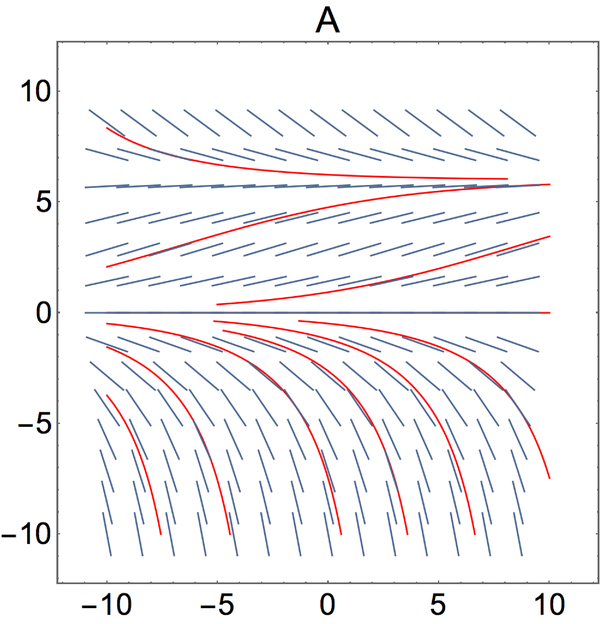
\includegraphics{direction_fields_A.png}
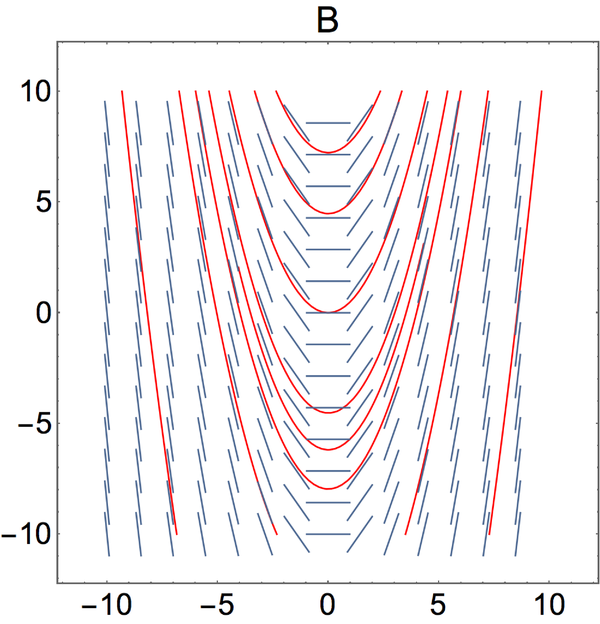
\includegraphics{direction_fields_B.png}
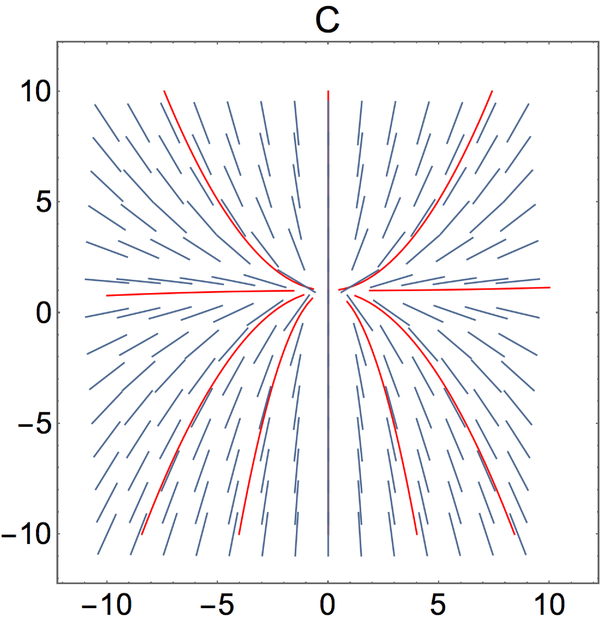
\includegraphics{direction_fields_C.png}

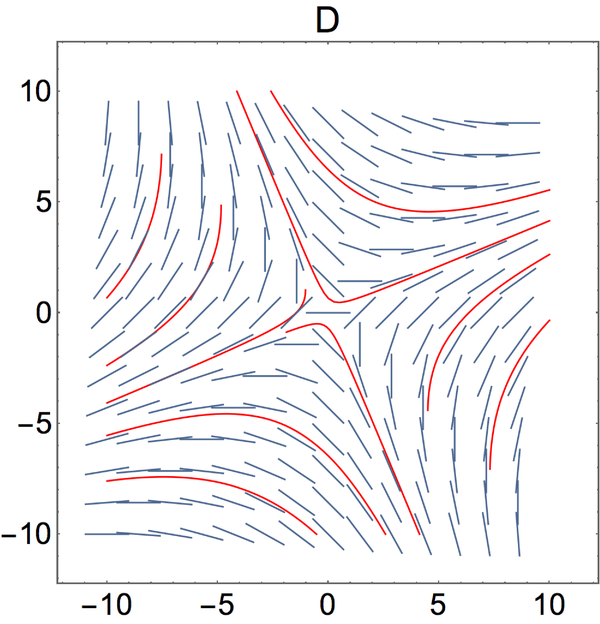
\includegraphics{direction_fields_D.png}
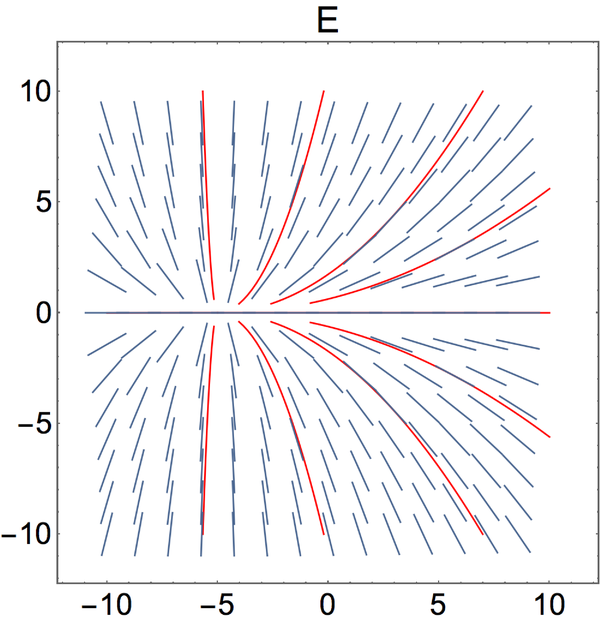
\includegraphics{direction_fields_E.png}
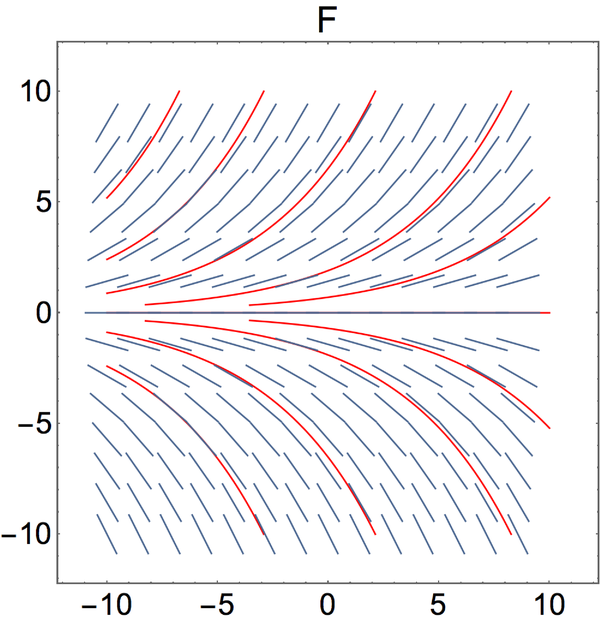
\includegraphics{direction_fields_F.png}

\subsection*{Solution}
\six{} (eg, ``abcdef'')

\hash{q}{743eb9}



%%%%%%%%%%%%%%%%%%%%%%%%%%%%%%%%%
\newpage
%%%%%%%%%%%%%%%%%%%%%%%%%%%%%%%%%
\section{Solving a simple 1st-order linear equation}

\subsection*{Resources}
\begin{itemize}
    \item Video: \url{https://www.khanacademy.org/math/differential-equations/first-order-differential-equations/differential-equations-intro/v/finding-particular-linear-solution-to-differential-equation}
\end{itemize}

\subsection*{Comment}
It's not easy to see when equations can be solved simply, like in the challenge below, and when they can not. But for a 1st-order linear differential equation, this method is often good to try first. If it's not 1st order and not linear, you know to try a different approach.

\subsection*{Challenge}
Determine the value of $y(x=1)$ for the following equation:

\begin{equation}
    y'=2y-5x+2
\end{equation}

\subsection*{Solution}
\six{}

\hash{u}{505c7b}




%%%%%%%%%%%%%%%%%%%%%%%%%%%%%%%%%
\newpage
%%%%%%%%%%%%%%%%%%%%%%%%%%%%%%%%%
\section{Separable equations I}

\subsection*{Resources}
\begin{itemize}
    \item Video I: \url{https://www.khanacademy.org/math/differential-equations/first-order-differential-equations/separable-equations/v/separable-differential-equations-introduction} 
    \item Video II: \url{https://www.khanacademy.org/math/differential-equations/first-order-differential-equations/separable-equations/v/particular-solution-to-differential-equation-example}
    \item Text:\url{http://tutorial.math.lamar.edu/Classes/DE/Separable.aspx}
\end{itemize}

\subsection*{Challenge}
Given the following equation:
\begin{equation}
    r' = -Sin(\theta)
\end{equation}
Determine the function $r(\theta)$ that passes through the point (0,1) in $\theta-r$ space, and then solve for $\theta = \pi/4$.


\subsection*{Solution}
\six{}

\hash{i}{7b35e2}




%%%%%%%%%%%%%%%%%%%%%%%%%%%%%%%%%
\newpage
%%%%%%%%%%%%%%%%%%%%%%%%%%%%%%%%%
\section{Separable equations II}

\subsection*{Resources}
\begin{itemize}
    \item Video I: \url{https://www.khanacademy.org/math/differential-equations/first-order-differential-equations/separable-equations/v/separable-differential-equations-introduction} 
    \item Video II: \url{https://www.khanacademy.org/math/differential-equations/first-order-differential-equations/separable-equations/v/particular-solution-to-differential-equation-example}
    \item Text:\url{http://tutorial.math.lamar.edu/Classes/DE/Separable.aspx}
\end{itemize}

\subsection*{Challenge}
Given the following equation:
\begin{equation}
    r' cot(\theta) + r = 2
\end{equation}
Determine the function $r(\theta)$ that passes through the point (0,1) in $\theta-r$ space, and then solve for $\theta = \pi/4$.

\subsection*{Solution}
\six{}

\hash{o}{87ee92}




%%%%%%%%%%%%%%%%%%%%%%%%%%%%%%%%%
\newpage
%%%%%%%%%%%%%%%%%%%%%%%%%%%%%%%%%
\section{Separable equations III}

\subsection*{Resources}
\begin{itemize}
    \item Video I: \url{https://www.khanacademy.org/math/differential-equations/first-order-differential-equations/separable-equations/v/separable-differential-equations-introduction} 
    \item Video II: \url{https://www.khanacademy.org/math/differential-equations/first-order-differential-equations/separable-equations/v/particular-solution-to-differential-equation-example}
    \item Text:\url{http://tutorial.math.lamar.edu/Classes/DE/Separable.aspx}
\end{itemize}

\subsection*{Challenge}
Given the following equation:
\begin{equation}
    y' x^2 - y = 0
\end{equation}
Determine the function $y(x)$ that passes through the point $x=2,y=1$ and then solve for the given $x$ value. State the value of $x$ where the solution is undefined. % Would be nice to couple this with a field graph.

\subsection*{Solution}
Solve for $x=4$:

\six{}

\hash{p}{09bb0e} 

Value of x where solution is undefined:

\six{}

\hash{a}{b30fe7} 




%%%%%%%%%%%%%%%%%%%%%%%%%%%%%%%%%
\newpage
%%%%%%%%%%%%%%%%%%%%%%%%%%%%%%%%%
\section{Compound increase}

\subsection*{Challenge}
If the amount of bacteria on a surface increases by 20\% every 25 hours, how much does the amount grow per hour in percentage terms? Ie, if one observes the amount of bacteria one hour from now, by what percentage should one expect the amount of bacteria to have increased?

\subsection*{Solution}
\six{\%}

\hash{s}{4288d8} 




%%%%%%%%%%%%%%%%%%%%%%%%%%%%%%%%%
\newpage
%%%%%%%%%%%%%%%%%%%%%%%%%%%%%%%%%
\section{Logistic equation}

\subsection*{Resources}
\begin{itemize}
    \item Videos: The 5 videos on the logistic differential equation and function starting at: \url{https://www.khanacademy.org/math/differential-equations/first-order-differential-equations/logistic-differential-equation/v/modeling-population-with-differential-equations}
\end{itemize}

\subsection*{Challenge}
Using the logistic equation, assuming an increase in the amount of bacteria measured in mg of 20\% every 25 hours, an initial amount of bacteria of 20 mg and a limiting amount of 400 mg, how much time, rounded to the nearest integer hours, must one wait to reach 300 mg of bacteria?

\subsection*{Solution}
\six{hours} (expressed as an integer)

\hash{d}{b0d406} 




%%%%%%%%%%%%%%%%%%%%%%%%%%%%%%%%%
\newpage
%%%%%%%%%%%%%%%%%%%%%%%%%%%%%%%%%
\section{Autonomous differential equations}

\subsection*{Resources}
\begin{itemize}
    \item Text: \url{http://tutorial.math.lamar.edu/Classes/DE/EquilibriumSolutions.aspx}
    \item Wikipedia: \url{https://en.wikipedia.org/wiki/Autonomous_system_(mathematics)}
\end{itemize}

\subsection*{Challenge}
Add the points of the autonomous differential equations in the following list:

1 point: $y' = cos(y)-5$

2 points: $y' = cos(y)/x - 5$

4 points: $y' = cos(y)/x - 5/x$

8 points: $y^2 = y' y+5$

16 points: $x y' = 5 y$

32 points: $y' = 1$

\subsection*{Solution}
\six{}

\hash{f}{9bf043} 




%%%%%%%%%%%%%%%%%%%%%%%%%%%%%%%%%
\newpage
%%%%%%%%%%%%%%%%%%%%%%%%%%%%%%%%%
\section{The stability of solutions I}

\subsection*{Resources}
\begin{itemize}
    \item Text: \url{http://tutorial.math.lamar.edu/Classes/DE/EquilibriumSolutions.aspx}
\end{itemize}

\subsection*{Challenge}
Considering the logistic equation $N'=0.2t(1-N/6)$, make 3 separate lists containing any equilibrium, semi-stable and unstable y-values.

To check your answer, sum the value of each list. If there are no values in a list, simply enter ``none'' to check the result.

\subsection*{Solution}
\subsubsection*{Equilibrium}
\six{}

\hash{g}{2c32d8} 

\subsubsection*{Semi-stable}
\six{}

\hash{h}{8b595d} 

\subsubsection*{Unstable}
\six{}

\hash{j}{4fd3f6}




%%%%%%%%%%%%%%%%%%%%%%%%%%%%%%%%%
\newpage
%%%%%%%%%%%%%%%%%%%%%%%%%%%%%%%%%
\section{The stability of solutions II}

\subsection*{Resources}
\begin{itemize}
    \item Text: \url{http://tutorial.math.lamar.edu/Classes/DE/EquilibriumSolutions.aspx}
\end{itemize}

\subsection*{Challenge}
Considering the differential equation $y'=(y^2-16)(y+3)^2$, make 3 separate lists containing any equilibrium, semi-stable and unstable y-values.

To check your answer, sum the value of each list. If there are no values in a list, simply enter ``none'' to check the result.

\subsection*{Solution}
\subsubsection*{Equilibrium}
\six{}

\hash{k}{667798} 

\subsubsection*{Semi-stable}
\six{}

\hash{z}{200aa3} 

\subsubsection*{Unstable}
\six{}

\hash{x}{d1ee5b}




%%%%%%%%%%%%%%%%%%%%%%%%%%%%%%%%%
\newpage
%%%%%%%%%%%%%%%%%%%%%%%%%%%%%%%%%
\section{Euler's method}

\subsection*{Resources}
\begin{itemize}
    \item Videos and exersizes in the ``Euler's Method'' section of Khan academy: \url{https://www.khanacademy.org/math/differential-equations/first-order-differential-equations/eulers-method-tutorial/v/eulers-method}
    \item Text: \url{http://tutorial.math.lamar.edu/Classes/DE/EulersMethod.aspx}
\end{itemize}

\subsection*{Challenge}
Considering the differential equation $y'=10-y$, an initial value of $y(0)=1$ and a step size of $\Delta x = 0.2$, use Euler's method to estimate the value of $y(x=1)$. The actual solution, $y(x)=10-9e^{-x}$, is shown below.

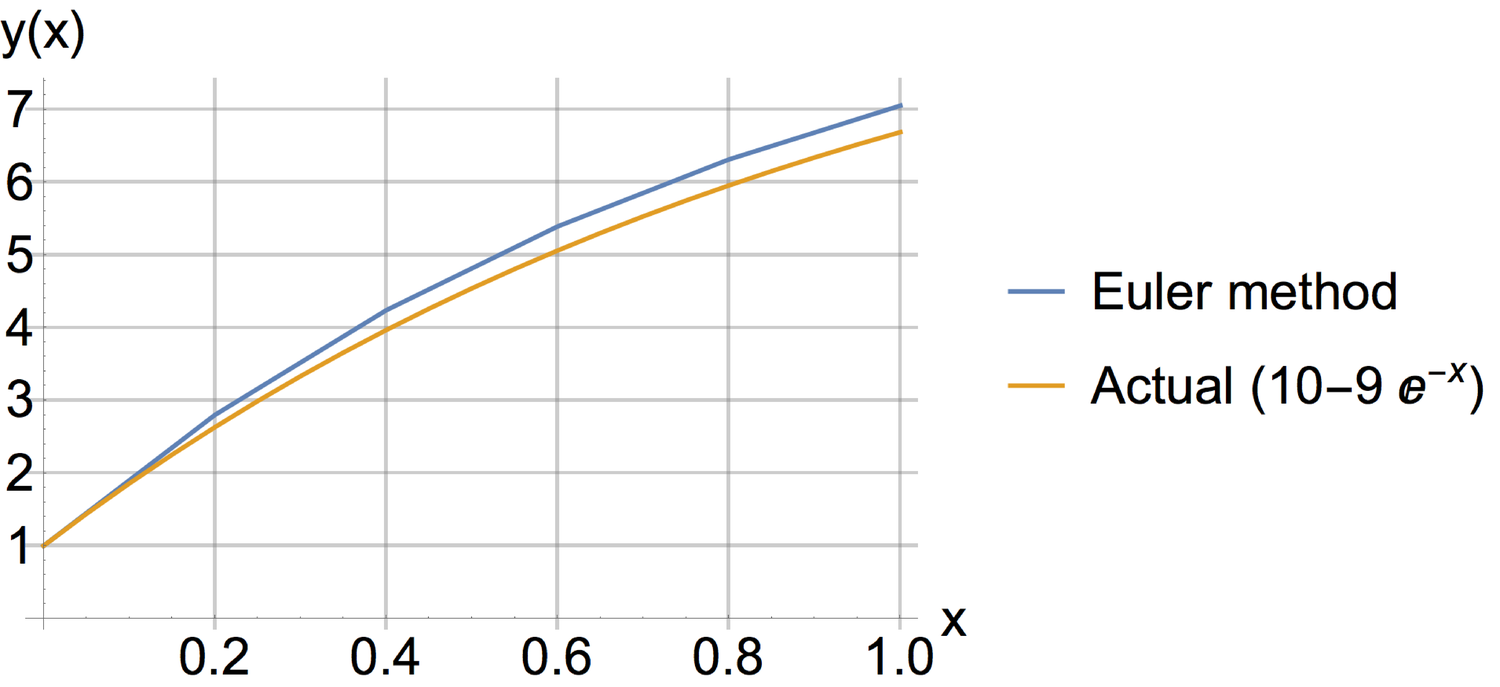
\includegraphics{eulers_method.png}

\subsection*{Solution}
\six{}

\hash{c}{1f90fa} 
% It would be nice to see if this error actually goes to zero in the end.


% Exact DE's
% If D[psi(x,y)] = \ldots, what is partial psi/partial x?
% Which of the following are exact differential equations? (points)
% About 4.5 weeks on 1st-order and 4.5 weeks on 2nd order?
% Khan covers 1st-order well but 2nd-order not so much.
% Follow Khan for 1st-order, then do 2nd order and fill in holes with Paul's notes - this may cause issues if terminology is different.
% More advanced topics are in Paul's notes, but first check how much time is remaining.

% Do I need to add more challenges for simple 1st order linear equations?
